\subsection{Prophet Interpreter}\label{subsec: prophet-interpreter}
prophet interpreter runs the prophet code in the field $\texttt{prophets}$ of program.Prophet interpreter does not change the status of PC and $\texttt{r}_{8}$.
It runs the prophet code and stores the status of context id in prophet segment of memory and update the PSP to free prophet memory in ascending order.
The prophet code snippet is as below, the entry procedure is the beginning when prophet interpreter run, the variable with prefix of $\texttt{cid}$ is the context id:
\begin{lstlisting}[label={lst:prophet-demo}]
%{
    function mod(felt x, felt y) -> felt {
        return x % y;
    }

    entry() {
        cid.r = mod(cid.x, cid.y);
    }
%}
\end{lstlisting}

The prophet interpreter illustration is as below.
The pink blocks are the logic relate to prophet interpreter.
The blue blocks are the logic relate to OlaVM executor.
The green blocks are the begin and end.
Prophet interpreter is embedded to OlaVMv executor as a module.
\ref{fig: prophet-interpreter-logic}:
\begin{figure}[!htp]
    \centering
    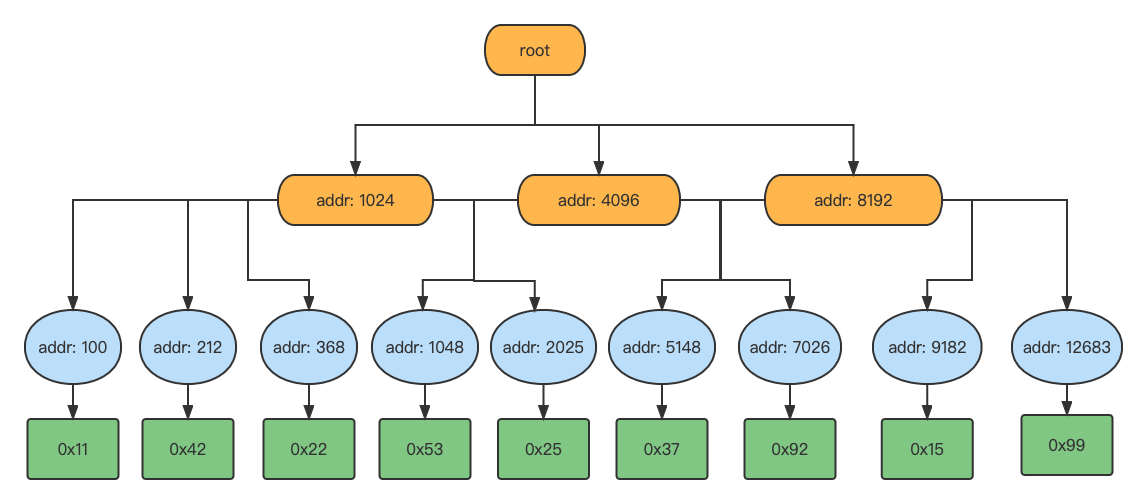
\includegraphics[width=0.8\textwidth]{memory-structure}
    \caption{OlaVM prophet interpreter flow}
    \label{fig: prophet-interpreter-logic}
\end{figure}
